% !TeX program = pdfLaTeX
\documentclass[smallextended]{svjour3}       % onecolumn (second format)
%\documentclass[twocolumn]{svjour3}          % twocolumn
%
\smartqed  % flush right qed marks, e.g. at end of proof
%
\usepackage{amsmath}
\usepackage{graphicx}
\usepackage[utf8]{inputenc}

\usepackage[hyphens]{url} % not crucial - just used below for the URL
\usepackage{hyperref}

%
% \usepackage{mathptmx}      % use Times fonts if available on your TeX system
%
% insert here the call for the packages your document requires
%\usepackage{latexsym}
% etc.
%
% please place your own definitions here and don't use \def but
% \newcommand{}{}
%
% Insert the name of "your journal" with
% \journalname{myjournal}
%

%% load any required packages here



% tightlist command for lists without linebreak
\providecommand{\tightlist}{%
  \setlength{\itemsep}{0pt}\setlength{\parskip}{0pt}}


% Pandoc citation processing
\newlength{\cslhangindent}
\setlength{\cslhangindent}{1.5em}
\newlength{\csllabelwidth}
\setlength{\csllabelwidth}{3em}
\newlength{\cslentryspacingunit} % times entry-spacing
\setlength{\cslentryspacingunit}{\parskip}
% for Pandoc 2.8 to 2.10.1
\newenvironment{cslreferences}%
  {}%
  {\par}
% For Pandoc 2.11+
\newenvironment{CSLReferences}[2] % #1 hanging-ident, #2 entry spacing
 {% don't indent paragraphs
  \setlength{\parindent}{0pt}
  % turn on hanging indent if param 1 is 1
  \ifodd #1
  \let\oldpar\par
  \def\par{\hangindent=\cslhangindent\oldpar}
  \fi
  % set entry spacing
  \setlength{\parskip}{#2\cslentryspacingunit}
 }%
 {}
\usepackage{calc}
\newcommand{\CSLBlock}[1]{#1\hfill\break}
\newcommand{\CSLLeftMargin}[1]{\parbox[t]{\csllabelwidth}{#1}}
\newcommand{\CSLRightInline}[1]{\parbox[t]{\linewidth - \csllabelwidth}{#1}\break}
\newcommand{\CSLIndent}[1]{\hspace{\cslhangindent}#1}

\usepackage{booktabs}
\usepackage{longtable}
\usepackage{array}
\usepackage{multirow}
\usepackage{wrapfig}
\usepackage{float}
\usepackage{colortbl}
\usepackage{pdflscape}
\usepackage{tabu}
\usepackage{threeparttable}
\usepackage{threeparttablex}
\usepackage[normalem]{ulem}
\usepackage{makecell}
\usepackage{xcolor}
\usepackage{siunitx}
\newcolumntype{d}{S[input-symbols = ()]}
\begin{document}


\title{Anti-Political Correctness and Authenticity Performances in
Politics in Brazil and the United States \thanks{The author declares no
competing interests.} }


    \titlerunning{Anti-Political Correctness and Authenticity
Performances}

\author{  Henrique Sposito \and  }

    \authorrunning{ Sposito }

\institute{
        Henrique Sposito \at
     Department of International Relations and Political Science,
Graduate Institute of International and Development Studies, Geneva,
Switzerland \\
     \email{\href{mailto:henrique.sposito@graduateinstitute.ch}{\nolinkurl{henrique.sposito@graduateinstitute.ch}}}  %  \\
%             \emph{Present address:} of F. Author  %  if needed
    \and
    }

\date{Received: date / Accepted: date}
% The correct dates will be entered by the editor


\maketitle

\begin{abstract}
Various politicians have publicly denounced ``political correctness''
(PC). While some scholars argue that anti-PC discourses in politics are
populist tools to label elites or a form of cultural backlash against
liberal changes, these explanations focus on specific manifestations of
anti-PC by specific politicians. Instead, this article argues that
anti-PC discourses are performances of authenticity in politics. As
authenticity performances, anti-PC discourses reduce the perceived link
between thinking and saying for audiences. A framework for identifying
several discursive performances of authenticity in politics that focuses
on displays (what), projections (who, when, and where), and mechanisms
(how) is developed. A purpose-built dictionary of terms is designed to
detect authenticity performances in text datasets of campaign rallies,
debates, interviews, and official speeches gathered for presidents and
presidential candidates in Brazil and the United States since the 1980s.
The analysis indicates that authenticities are not performed more
frequently in election years, politicians usually perform different
authenticities most when they are candidates or after having left
office. Although, in the case of Brazil, authenticity performances
spiked from 2011 to 2016 while Dilma Rousseff was in office. The types
of authenticity performed over time also changed in each case across
time, indicating that contextual conditions make some types of
performances more, or less, credible to audiences and that politicians
adapt to perform what audiences ``want to hear''. Lastly, debates have
become the setting in which authenticity is performed most frequently,
whereas interviews are the setting in which authenticity is performed
least frequently, in both cases in recent years.
\\
\keywords{
        authenticity \and
        political correctness \and
        pollitically correct \and
        performance \and
        Brazil \and
        United States \and
    }


\end{abstract}


\def\spacingset#1{\renewcommand{\baselinestretch}%
{#1}\small\normalsize} \spacingset{1}


\hypertarget{introduction}{%
\section{Introduction}\label{introduction}}

In the second sentence of his inaugural speech as president of Brazil,
Jair Bolsonaro declared the day in which the people began to be free
from political correctness \footnote{ Find the whole speech
  \href{https://www.youtube.com/watch?v=5iPVlE_9kFw}{here}. Besides
  denouncing PC, Bolsonaro has also frequently referred to indigenous
  peoples and LGBT community in politically incorrect ways.}. Bolsonaro
is not unique in this sense, politicians as Trump, Chavez, Morales,
Berlusconi, Bush, Sanders, and Lula, have openly denounced political
correctness (PC) \footnote{ PC is used as an abbreviation for political
  correctness and politically correct throughout the paper, that is, as
  a noun and as an adjective.} and/or publicly employed politically
incorrect language \footnote{ Trump denounces PC and employs politically
  incorrect language across several domains ranging from immigration to
  race and indigenous people. Trump's `war' on PC is frequently brought
  up in campaign
  \href{https://edition.cnn.com/2018/10/30/politics/donald-trump-hate-speech-anti-semitism-steve-king-kevin-mccarthy/index.html}{rallies}
  and on
  \href{https://www.thetrumparchive.com/?searchbox=\%22politically+correct\%22}{Twitter}.
  Morales displays `bad manners', favors plain speaking and is not PC
  often making sexist and homophobic
  \href{https://www.bbc.com/news/world-latin-america-34851896}{comments}.
  When it comes to Hugo Chavez, the leader making public sexual comments
  during his talk show aired on national television, towards George W.
  \href{https://www.youtube.com/watch?v=lOsABwCrn3E}{Bush}, among many
  others controversial
  \href{https://elpais.com/internacional/2013/03/06/actualidad/1362528053_830886.html}{remarks}.
  Berlusconi has numerous times made references to Barack Obama's skin
  \href{https://www.theguardian.com/world/2009/sep/28/obama-tan-berlusconi}{color}
  in incorrect ways, made similar comments about some football
  \href{https://www.si.com/soccer/2013/02/06/mario-balotelli-racism-ac-milan}{players},
  and made several sexist and homophobic public
  \href{https://time.com/5179379/italy-silvio-berlusconi-sexist-remarks-women/}{remarks}.
  Lula quickly recalled the national guide on PC language as he
  constantly used several of the expressions listed in his speeches and
  campaign
  \href{https://www1.folha.uol.com.br/folha/brasil/ult96u68810.shtml}{rallies}.
  Bush, while president, famously denounced PC language on campuses
  during a commencement
  \href{https://www.youtube.com/watch?v=4IORaF6fi_Y}{speech}. Bernie
  Sanders stated several times how important PC was for Trump's campaign
  and PC had gone too
  \href{https://qz.com/865263/bernie-sanders-and-political-correctness-democrats-are-learning-all-the-wrong-lessons-from-donald-trump-election-win/}{far}.}.
Broad audiences appear to respond positively to these statements in
multicultural countries, such as the United States (US) and Brazil,
where large portions of the population fall under racial, ethnic, and
other categories PC language attempts to safeguard \footnote{ Most
  Americans appear unsupportive of PC language with estimations that
  range from 52\% of the population (Montanaro 2018) to 80\% of the
  population disliking PC (Mounk 2018). This change in percentages
  derives from the type of questions asked. For example, one poll asked
  if participants thought that PC was a big issue in the US, while
  another asked if they favored the process of the country becoming more
  politically correct. For Brazil, a recent national poll asked
  participants whether they agreed that the `PC patrol is making the
  world too boring', 56\% of participants agreed completely or partially
  with the statement (Goncalves and Goncalves 2020).}. Populist scholars
argue that contemporary populists' profit from breaking with PC language
and use PC to identify modern elites (see Mudde 2004) \footnote{ To
  discuss whether, or the extent which, Bolsonaro or Trump are populists
  is not the objective of this paper, though there are many excellent
  discussions on this topic (see Tamaki and Fuks 2020; Hawkins and
  Rovira Kaltwasser 2018).}. Cultural backlash scholars argue that
anti-PC discourses speak to resentment caused by silent liberal changes
(see Norris and Inglehart 2019). However, both populism and cultural
backlash focus on specific manifestations of these discourses by
specific leaders that embody their arguments, leaving aside any
systematic or empirical analysis of language usage or patterns across
contexts. \emph{How, then, do anti-PC discourses appear and change over
time in politics?}

This paper argues that anti-PC discourses in politics are performances
of authenticity. Performances are the projections of definitions of a
situation to others (see Goffman 1956; Alexander, Giesen, and Mast
2006). Authenticity, as a perceived character trait that conveys ones'
convictions, is connected to higher levels of political trust from
electorates (Stiers et al. 2021; Valgarosson et al. 2021) and is
essential to a candidate's political success (see Alexander 2010;
Fordahl 2018). As an authenticity performance, anti-PC language reduces
the perceived link between thinking and saying to audiences (see Conway
et al. 2009; Conway, Repke, and Houck 2017). There are, though, other
political performances that can generate an authenticity perception in
audiences. This article, therefore, develops a framework to identify
various types of authenticity performances in political discourses. The
framework focuses on the performative display (what), the projection
(who, when, and where), and the mechanisms (how). Authenticity
performances are divided into two types, individual and collective.
Individual authenticity performances derive plausibility from audiences'
expectations about a political performer. These performances include
claims of truth telling, lie accusations, taking responsibility for
actions, or pointing fingers at other politicians' mistakes. Collective
authenticity performances derive plausibility from the shared cultural
knowledge between politicians and audiences. These include references to
origins, allusions to common sense, anti-PC discourses, or assertions of
territorial knowledge.

Political discourses at the national level in Brazil and the US since
the 1980s were gathered and explored to assess variations over time, by
politicians, and across different settings. The 1980s were chosen as the
starting point as they mark the beginning of the university debates
surrounding PC language in the US and the decade in which democracy was
re-established in Brazil. Texts for campaign rallies, debates,
interviews, and official speeches for presidents and presidential
candidates in Brazil and the US until December 2021 were scraped to
construct the datasets. A purpose-built dictionary of terms was created
to capture various authenticity performances, as anti-PC, in discourses.

The findings indicate that the frequencies of authenticity performances
are not systematically greater in election years. Usually, politicians
perform authenticities above the 95th percentile when they are
candidates, before being elected a first time, or after having left
office. However, in the case of Brazil, we see a spike in the frequency
authenticity is performed in politics from 2011 to 2016, the Dilma
Rousseff years in office. Women in politics, arguably,perform
authenticity to justify themselves and their public policy choices more
frequently than the men in the sample. Moreover, the variation in types
of authenticity performed over time and across cases indicates that
contextual conditions make some performances more, or less, credible to
audiences at certain junctures. Indeed, many authenticity performances
appear in high frequencies for opposing, and associated, candidates in
similar years as is the case of anti-PC performances in Brazil in the
mid-1990s. Politicians, thus, adapt to perform authenticities audiences
``want to hear''. Finally, debates have became the setting in which
authenticity is performed most frequently, whereas interviews are the
setting in which authenticity was performed the least frequently, in
both cases in recent years. Debates are large-scale media events that
produce ``sticky'' political bites charged with imagery that circulate
to mark election cycles in these democracies. Whereas social media
platforms give politicians diverse outlets to interact directly with
audiences, bypassing journalists in interviews.

\hypertarget{pc-anti-pc-populism-and-backlash}{%
\section{PC, Anti-PC, Populism, and
Backlash}\label{pc-anti-pc-populism-and-backlash}}

\hypertarget{pc-and-anti-pc-overview-and-effects}{%
\subsection{PC and anti-PC overview and
effects}\label{pc-and-anti-pc-overview-and-effects}}

Definitions of PC range from an ``idealistic intervention'' to ``liberal
fascism'' (Hughes 2011; Feldstein 1997). In practice, PC language avoids
judgmental terms, preferring euphemistic substitutions and it
presupposes that lexicon changes mediate discrimination in positive ways
(Hughes 2011, 13) \footnote{ For a good discussion of lexicalization and
  language change in linguistics, refer to Brinton and Traugott (2005).
  For a discussion on the complexities involved in why language changes,
  and not, as well as how meaning might be affected by such changes
  refer to Bybee (2015)}. Anti-PC discourses, instead, represent a
\emph{dismissal of PC substitutions and/or the denouncing of PC language
and users}. However, to understand what anti-PC language entails, we
must first briefly overview PC's history and effects. The modern
conception of PC originated in Mao Tsé-Tung's depiction of the `correct'
socialist party line in the 1930s, used to describe doing the right
things and thinking the right thoughts (Hughes 2011). The term was
picked up by leftist circles in the US during the 1960s and used to
describe more orthodox followers of socialism or as a critique of
excessive orthodoxy (Feldstein 1997; Weigel 2016; Hughes 2011). It was
not until the 1980s that right-leaning conservative elites in the US,
including many academics, started denouncing PC language substitutions
as a left leaning strategy that restricted freedoms of speech (Feldstein
1997; Weigel 2016). These conservative elites were able to swiftly
recycle the meaning of PC by keeping some of its' original meaning, but
disconnecting it from historical context, and conflating it with enemy
building narratives and imagery (Feldstein 1997).

The university debates in the 1980s and 1990s brought wide attention to
PC, multiculturalism, and affirmative action in the US (Berman 2011).
D'Souza (1991), for example, discussed the apparent duplicity between a
liberal educational system and multicultural claims, arguing that PC
further victimize minorities on campuses and undermine their merits with
affirmative action policies that could potentially generate more racist
backlash. As a response, Gutmann and Habermas highlighted how misplaced
PC debates politicized and polarized important societal dialogues
(Gutmann 1994). Yet, most multiculturalism scholars at the time dealt
with PC as a matter of public or party disagreement and lamented their
popularity with certain communities while leaving unaddressed the nature
of PC language, the relation between the speaker's identity to the
information provided, and why diverse communities related or contested
semantic changes (Loury 1994). The university debates helped disseminate
and connect matters of PC, affirmative action policies, and
multiculturalism to left leaning (progressive) political ideologies and
anti-PC to right-wing (conservative) ideologies across the world
(Feldstein 1997; Bush 1995). By the mid-1990s, PC debates in the US had
become as much about rhetorical strategies to forward ideological
political agendas as about the diverse cultural movements' efforts to
re-label (Feldstein 1997; Hall 1994).

The spreading of issues covered by PC language and the complex political
forces supporting, and opposing, it required that the cultural and
individual effects of PC in society be theorized. Hall (1994), for
example, describes the ambiguous truth and contested cultural authority
of the PC phenomenon to argue that individuals may disapprove of PC
language because these are relatively new demands for cultural
transformation. Similarly, Fairclough (2003, 24) argues that PC is a
socially constructed cultural and political label for which effects
depend on the resistance of structure and practices. Even though
euphemistic substitutions are not a modern manifestation, as changing
orthodoxies under moral imperatives exist since the invention of
printing, PC language has expanded the number of substitutions (Hughes
2011). This expansion of PC language generates more abstract and
imprecise replacements that can feel unnatural, create confusion,
patronize subjects, and further socioeconomic inequalities via
linguistic processes (Hughes 2011). This contributed to the evolution of
PC from a noun used to describe language substitution to an adjective
used to describe excess politeness or evasion of truths in society or
for individuals (Weigel 2016; Chait 2015).

\hypertarget{anti-pc-populisms-and-cultural-backlash}{%
\subsection{Anti-PC, populism(s), and cultural
backlash}\label{anti-pc-populisms-and-cultural-backlash}}

In \emph{The Populist Zeitgeist}, on the rise of populist parties in
liberal democracies, Mudde (2004, 543) defines populism as a thin
centered ideology. There are three mentions of PC in the article
discussing how contemporary populists profit from breaking with
politically correct language, because citizens' increased emancipation
made issues surrounding PC more widespread, alongside how PC has been
used to identify a modern elite (Mudde 2004, 594--602). Since then,
populists have routinely been associated with anti-PC discourses. Still,
Mudde's analysis leaves undertheorized which elites are characterized as
PC by various populist leaders with a variety of ideological
commitments. This is puzzling since political, economic, and
intellectual elites are often the drivers of anti-PC discourses in
societies. Moreover, if populism is not a standalone ideology (see Mudde
2007), it is hard to pinpoint if anti-PC discourses are a portion or
manifestation of the populist (thin)ideology, an adjacent ideology, or a
contextual feature of a specific society \footnote{ See Aslanidis (2016)
  for a good discussion on whether populism is an ideology.}. Besides,
the account leaves unclear when, and why, anti-PC discourses are a
politically profitable strategy for populists but not for other
political actors. Other influential theories of populism do not mention
anti-PC discourses (see Weyland 2001; Laclau 2005; Hawkins 2009) and,
when mentioned, anti-PC discourses fulfill a peripheral role to help
identify exclusionary right-wing populist parties in Europe (Betz 2001).
In such, there appears to be a leap associating populism with anti-PC
discourses without systematically or empirically analyzing its usage in
time and patterns across contexts.

Recent efforts to rethink populism as a political performance or a
repertoire focus on patterns of communication in populism. For instance,
Moffitt and Tormey (2014) (p.~387) argue that we must rethink populism
as ``the repertoires of performance that are used to create political
relations''. More specifically, we must think about how populists
perform ``the people'', threats, breakdowns and crisis, and bad manners
(Moffitt and Tormey 2014; Moffitt 2016). Concerning bad manners, the
authors argue that ``much of populists' appeal comes from their
disregard for `appropriate' ways of acting in the political realm''
(Moffitt and Tormey 2014, 392). Bad manners often performed with
swearing, slang words, and political incorrectness (Moffitt and Tormey
2014, 392). Performing these repertoires helps politicians appear as an
``outsider'' against the ``establishment'' (Moffitt and Tormey 2014;
Moffitt 2016). Likewise, arguing against a pure definition of populism,
Brubaker (2020, 60) contends that populism is a discourse and stylistic
repertoire that includes ``a communication style that claims to favor
plain-speaking, common sense and authenticity against intellectualism
and political correctness''. Anti-PC discourses might be a portion of a
broad populist communication style or repertoire, although favoring
plain speaking, displaying bad manners, or being anti-PC are not
exclusive to populists or connected to populist discourses by ideology
\footnote{ Brubaker (2017) view of anti-PC discourses is not
  inconsistent with Mudde (2004) point about PC and elites (see Brubaker
  2020; Mudde 2007). Rather it implies that certain intellectual elites
  might be tagged as PC, not any ``modern'' elite, and this is connected
  to anti-intellectualism. This is also consistent with Hughes (2011)
  argument about PC language expansion that leaves some people feeling
  patronized and confused by PC language.}.

At the intersection between populism, authoritarianism, and
multiculturalism, \emph{Cultural Backlash} argues that authoritarian
populists appeal to more conservative portions of the population, who
feel ignored seeing their societies shift towards post-materialism
(Norris and Inglehart 2019). There are eight mentions of PC in the book.
On anti-PC, the authors argue that social conservative individuals with
authoritarian orientations react to some trends with feelings of
resentment for the erosion of respect for their core values and that
``is the essence of the backlash against `political correctness', in
which sexist language, anti-foreigner sentiments, or the expression of
racist attitudes are condemned by the liberal consensus and silenced in
mainstream political debate'' (Norris and Inglehart 2019, 123). Rather
than developing further the mechanisms of how anti-PC discourses work,
deliberate on which types of anti-PC discourses connect to resentment,
the authors take for granted that anti-PC discourses are connected to
resentment, and that is why they resonate with ``old, rural, or
uneducated'' electorates \footnote{ Norris and Inglehart (2019) appear
  to `passively' pass on the blame to `old, rural, and uneducate' voters
  for `undesirable' political outcomes with broad causal explanations
  extrapolated from thin linear correlations that illustrate little of
  the complex relationships theorized. Others, as Mishra (2017),
  sometimes rely on a misplaced engagement with history that focus on a
  few instances that exemplify arguments as if these were the rule.}.
Even so, anti-PC discourses appear to resonate more broadly within
societies for various reasons, many unrelated to resentment (e.g.~humor)
\footnote{ There are countless examples of PC and anti-PC language being
  explored in humoristic ways for entertainment as, for example,
  notoriously, TV shows as `South Park', `The Office', and `It's Always
  Sunny in Philadelphia'.}. How Bolsonaro, for example, employs anti-PC
in quick, direct, and short comments that focus on culturally salient
themes without being necessarily internally coherent is, arguably, more
decisive to his following than the content itself (Carlo and Kamradt
2018). Or how Trump is characterized as `not being PC', as a character
trait, appears more decisive to voters than his recognizable flaws or
the negative meanings associated to what he says \footnote{ Bill Maher,
  a journalist and comedian who was the host of a television series
  called Politically Incorrect in the 1990s,
  \href{https://www.youtube.com/watch?v=CCQ3VyKe1Vs}{contends} that
  `when you talk to Trump supporters, they're not blind to his myriad
  flaws, but they always say he is not politically correct'.}. While
both the cultural backlash and populism accounts of anti-PC in politics
have merits, they focus on a few specific manifestations of these
discourses by particular leaders that embody their respective arguments.
Consequently, these literatures only partially explain what anti-PC
discourses are, how they function, or why they matter for political
outcomes.

\hypertarget{theory}{%
\section{Theory}\label{theory}}

\hypertarget{performance-authenticity-and-anti-pc-in-politics}{%
\subsection{Performance, authenticity, and anti-PC in
politics}\label{performance-authenticity-and-anti-pc-in-politics}}

Performances are the projections of a situation when one appears before
others, ``however passive their role may seem to be, will themselves
effectively project a definition of the situation by virtue of their
response to the individual'' (Goffman 1956, 3). But why should we
understand discursive politics through performance or, rather, why do
politicians say the things they do? Conventionally, there are two
answers to this question. On the one hand, politicians might say the
things they do according to what is more profitable to them
(i.e.~rational choice). On the other hand, politicians might say the
things they do because of their beliefs (i.e.~ideology). Though, neither
may hold in practice as politicians can, at different times, say what is
more profitable, say what they believe in, or say things without
intentionally thinking about it. Normally, whether a politician is
saying what they believe in, or what is more profitable, depends on the
audiences' interpretation. Understanding politics through performance
offers a more flexible answer to why politicians say the things they do:
to project their understandings (see Alexander 2011). Performance allows
to theorize that audience's interpretation hinges on factors beyond
discursive content or meaning, such as how things are said (see
Alexander, Giesen, and Mast 2006; Alexander 2011). Seeing politics
through performance provides more realistic assumptions to theorizing
how politicians ``do politics'' (see Van Dijk et al. 1997).
Understanding politics through performance focus less on causality and
interpretation of message meaning in discourse and more on identifying
discursive patterns and functioning (see Alexander 2011; Alexander,
Giesen, and Mast 2006).

Capturing audience's perception and other discursive elements beyond
text is challenging. There are, however, several capturable discursive
displays connected to the how, the where, and the when of political
performances that allow to identify patterns and variation in political
performances as the performer's role, the script, the stage, and the
audience, rather than the meanings associated with the content of a
political discourse. There are also important implications of thinking
discursive politics through performances. Performance places agency both
with audiences, watching and evaluating politicians ``doing'' politics,
and with political performers (see Alexander 2011). This means script
changes can be theorized to be intentional individual innovations or
unintentional chattering by performers, while political accomplishments
reflect positive evaluations from audiences. This does not mean factors
such as social media, economic crisis, and cultural changes, among
others, are irrelevant. Instead, these become background representations
to be explored in political scripts and provide context for audiences'
interpretation (see Alexander 2011).

Authenticity has long been discursively performed in politics with, for
example, self-references to origins, remarkable stories, allusions to
civic tradition, and displays of `vulgarism' (Fordahl 2018, 309;
Alexander 2010). Authenticity is an individualistic performance that
aims at radiating truthfulness outwards (Taylor 1992; Fordahl 2018).
Authenticity in politics does not concern being truthful to oneself but
appearing coherent with individual or societal values to audiences
(Valgarosson et al. 2021; Fordahl 2018). Stiers et al. (2021) refer to
authenticity in politics as an essential character trait that conveys
candidates' convictions and that has positively affected electoral
preferences across several European democracies. As a political tool,
authenticity helps build political trust for candidates by demonstrating
to electorates that politicians are in touch with ordinary people and
their struggles (Valgarosson et al. 2021). Authenticity perceptions
were, for example, essential for Obama's success in 2008 (Alexander
2010) and, arguably, defined the 2016 American election in Trump's favor
(Fordahl 2018). Authenticity, in politics, is an unstable and malleable
label that requires social validation while demanding contortion,
modification, and active individual effort (Fordahl 2018).

As a communication norm, PC language attempts to remove negative
language by means of self and group censorship (Conway et al. 2009;
Conway, Repke, and Houck 2017). This communication norm can backfire due
to contamination of individual information processes by authority or
legitimacy effects (Conway et al. 2009; Conway, Repke, and Houck 2017).
Authority effects surrounding PC language occur when language is
believed to be insincere if it is commanded by an authority (Conway et
al. 2009). Legitimacy effects are caused by individuals' own
self-censorship, which leads to increased awareness that language
interactions may not be genuine (Conway et al. 2009). Building on these
findings, Rosenblum, Schroeder, and Gino (2020) use several survey
experiments to illustrate how politically incorrect language makes
political communicators appear more authentic, have stronger
convictions, and be less strategic, in comparison to PC politicians. In
fact, the denouncing of a ``PC politician'' or a ``PC ideology''
engrains an allusion to inauthenticity, to someone or something that
expresses its views in calculated ways to avoid judgment (Hughes 2011;
Weigel 2016). Anti-PC discourses are connected to authenticity in
politics by reducing the perceived link between thinking and saying for
audiences (see Conway, Repke, and Houck 2017) \footnote{ The argument
  also considers the insights of bad manners as a repertoire (Moffitt
  2016; Moffitt and Tormey 2014) of plain speaking as communication
  style (Brubaker 2020, 2017) in populism. Though the conceptualization
  here is broader and intends to theorize anti-PC outside of populism,
  it is somewhat consistent with how these theorists understand what
  these repertoires/styles are, how they work in politics, and why they
  might matter.}. Anti-PC performances signal to audiences' precisely
that politicians might be coherent to an inner self. Though,
authenticity in politics can be performed in politics in several
additional ways.

\hypertarget{authenticity-performances}{%
\subsection{Authenticity performances}\label{authenticity-performances}}

Valgarosson et al. (2021) argue that there are three broad types of
authenticities, historic, categorical, and value authenticity (i.e.~the
authentic politician); value being the most pertinent in politics.
Stiers et al. (2021) associate authenticity in politics to a sense of
``realness'' that, in recent times, has repeatedly turned to
anti-politics to connect politicians with ordinary people. The authentic
politician is an abstract individual trait or group perception, with
broad political implications. How does authenticity come about in
politics? Looking at authenticity in politics, as a performance,
requires identifying displays, projections, and mechanisms. Display
concerns detecting a certain performance (what) and is constrained by
projection and mechanism. Projection relates to the level at which it is
convincing that a performance is authentic. Projection encapsulates the
role (who), the setting (where), and the structure (when) for certain
display(s). The role relates to the part a performer takes in politics.
Roles can generate different expectations and ranges of possibilities
for authenticity performances (e.g.~candidates versus elected
officials). Setting refers to where a performance takes place
(e.g.~debate or official speech). Structure indicates the timing in
which performance is inserted (e.g.~before/after an election).
Mechanisms refer to the theorized pathways (how) by which a projected
display might work to produce authenticity. Diverse answers to each of
these performative aspects generate different expectations about
authenticity performances in politics.

Although what could be an authenticity performance is not always
straight forward or capturable discursively, there are several
indications of how authenticity has been previously performed
dscursively in politics. Alexander (2010), for example, discusses how
allusions to origins, territory, and civic traditions were employed by
Obama to connect with audiences and generate a sense of authenticity.
These performances focus on the cultural connections shared by
politicians and audiences and are essential to legitimize a candidate's
knowledge about the ``real'' issues people in the country face. Fordahl
(2018) argues that Trump's authenticity was built upon iconic, often
vulgar, representations of American life and reality performed
consistently from his ``straight shooter dealmaker'' role. Allusions to
traditional national values and his business experience were central to
Trump's performances. These noticeable types of performances in
discursive politics are authenticity performances, which can be divided
in two types: \emph{individual} and \emph{collective}. The types refer
to the mechanism that might give plausibility to a certain performance.
Individual authenticity performances derive plausibility for performance
based on audiences' expectations about a political performer (or
opponent) considering the information they have. These performances
include stating to be telling the truth, claiming others are lying,
taking responsibility for actions, or pointing fingers at other's
errors. Collective authenticity performances are more elaborate displays
of authenticity that derive plausibility for performance based on the
cultural connections shared between audiences and performer. These
performances include anti-PC \footnote{ Politically incorrect
  expressions coded in dictionary were selected from a 1992 dictionary
  of politically correct language, this assumes that most of these terms
  have for long been agreed upon as not PC (Beard and Cerf 1993).},
pointing at origins, allusions to common sense, or claims of territorial
knowledge. Table 1, below, summarizes each authenticity performance
theorized, the type, their respective displays, and mechanisms.

\begin{landscape}

\begin{table}

\caption{\label{tab:Table 1}Authenticity Performances, Displays, and Mechanisms}
\begin{tabu} to \linewidth {>{\raggedright\arraybackslash}p{3 cm}>{\raggedright\arraybackslash}m{3 cm}>{\raggedright\arraybackslash}m{6 cm}>{\raggedright\arraybackslash}m{3 cm}}
\toprule
Authenticity Performance & Type & Displays & Mechanism\\
\midrule
\textbf{Truth Telling} & Individual & Mentions truthfulness, sincerity, and honesty when describing oneself. Examples: 'the truth is', 'this is the truth', 'am not lying', 'is/are/am honest', 'honesty', 'is/are/am sincere', 'is/are true' & Speaker appears to be telling the truth regarding their beliefs or facts - Individual.\\
\textbf{Lie Accusations} & Individual & Mentions dishonesty, untruthfulness, and insincerity when used to describe others. Examples: 'not the truth', 'not true', 'untruthful', 'is/are lying', 'is/are liars', 'is/are dishonest', 'is/are fake', 'is/are a hypocrite' & Speaker appears more sincere vis-a-vis others - Individual.\\
\textbf{Consistency} & Individual & Mentions career consistency, responsibility, accountability for individual. Examples: 'I/we delivered', 'check and see', 'keep my word', 'keep promises', 'I am/we are responsible', 'I/we take responsibility', 'I/we guarantee' & Speaker appears consistent regarding pledges - Individual.\\
\textbf{Finger Pointing} & Individual & Mentions lack of accountability, inconsistency and/or blame others for mistakes. Examples: 'are/is inconsistent', 'are/is irresponsible', 'their fault', 'not my fault', 'they left us with', 'are/is responsible', 'costed us', 'false/fake/broken promises' & Speaker appears not accountable for previous undesirable outcomes - Individual.\\
\textbf{Origins} & Collective & Alludes to birthplace, origins, and roots to describe background, values, and tell their story. Examples: 'I was born in', 'I come from', 'I/we grew up in', 'my family', 'I was raised', 'my background', 'I was thought', 'my hometown/community/city' & Speaker seems culturally connected to the nation - Collective.\\
\addlinespace
\textbf{Common Sense} & Collective & Alludes to common sense, reason, and logic to describe choices or preferences. Examples: 'is/are common sense', 'everyone/everybody knows', 'it is undeniable', 'stating the obvious', 'everyone agrees', 'we all know', 'no one disagrees that', 'we have all learned that' & Speaker seems to make choices consistent with what others in society would do - Collective.\\
\textbf{Territory} & Collective & Alludes to sub-portions of the territory known and/or visited. Examples: 'have seen in', 'have been to', 'I/we/have visited', 'came all the way to', 'came/came back from', 'saw/see first-hand in', 'I/we were hosted', 'my/our time in' & Speaker seems territorially connected to sub-regions, regions, or national territory - Collective.\\
\textbf{Anti-PC} & Collective & Alludes to PC language negatively, employs politically incorrect language, or claims to speak what one thinks without filters. Examples: 'not politically correct', 'political correctness', 'speak/speaking my mind', 'say/saying what everyone thinks', 'colored/oriental/fat/handicapped people' & Speaker seems to be saying what thinks on culturally contested themes - Collective.\\
\bottomrule
\end{tabu}
\end{table}

\end{landscape}

\hypertarget{methodology}{%
\section{Methodology}\label{methodology}}

\hypertarget{case-selection}{%
\subsection{Case selection}\label{case-selection}}

In Brazil, restrictions to freedoms of speech based on racism were
criminalized in the constitution of 1988 while affirmative action
policies in universities were put in the late-1990s. Although these were
widely discussed in society, albeit a long history of direct and
indirect political opposition to them, neither constitutional nor
affirmative action debates sparked much discussion about PC (see Farias
2001; Freitas and Castro 2013). In fact, the PC terminology was
translated from outside Brazil (Possenti 1995) and it did not directly
appear in public debates until 2004, when the Secretariat of Human
Rights of the President published a manual of PC language which
contained 96 popular expressions deemed incorrect for being racist,
sexist, or homophobic (Fiorin 2008; Morato and Bentes 2017). A that
time, the federal government quickly recalled the publication due to
internal opposition and external backlash (Fiorin 2008; Morato and
Bentes 2017). Since the mid-2000s humoristic interpretations of
politically incorrect language and politically charged calls against a
PC country started to appear frequently in the Brazilian media (Morato
and Bentes 2017; Weinmann and Culau 2014). Alongside this, several
articles in popular periodicals and popular books were written opposing
PC language (Weinmann and Culau 2014). By the 2010s, PC started to be
referred to as a ``controversy'' and, nowadays, PC in Brazil is a widely
contested phenomenon in society and politics.

Apart from that, Brazil and the US held the world's largest slave
populations until slavery was abolished respectively in each country.
Similarly, the two countries became large settler states for diverse
groups of migrants in the following centuries. These historical
processes rendered their current populations heterogenous in terms of
demographic composition and cultural heritage. This explain the
appearance and influence of PC language in these societies, but the
eminence of anti-PC discourses in national politics is somewhat puzzling
as electorates are likely to encompass several large groups that PC
language safeguards. While Brazil and the US are relatively similar in
geographical and population sizes, they are dissimilar in many other
ways including levels of economic development, culture and, in some
ways, their political systems. Thus, each case is understood as a
configuration, formed by the aggregation of parts that make sense in the
context of each case (Ragin 1987). This allows us to consider
similarities and differences across time and space and broadly compare
them in many aspects, including political discourses.

\hypertarget{data}{%
\subsection{Data}\label{data}}

Text data on official speeches, campaign rallies, debates, and
interviews for elected presidents and runoff candidates were gathered
since 1980 for the US and 1985 for Brazil. In the US, the 1980s marked
the beginning of the university debates surrounding PC. In Brazil,
democracy came back in 1985, though direct presidential elections were
held in 1989. All the texts for the US were scraped from
\href{https://www.presidency.ucsb.edu}{The American Presidency Project}
repository (TAPP). Collecting data for Brazil proved more difficult due
to availability. For official speeches, Cezar (2020) dataset on official
speeches for Brazilian presidents from 1985 to 2019 was updated to
include the missing speeches from 2019 to 2021 using the
\href{http://www.biblioteca.presidencia.gov.br/sobre-a-biblioteca/biblioteca-da-presidencia-da-republica}{Brazilian
Presidential Library}. Text for debates, interviews, and campaign
rallies were scraped from subtitles automatically generated for YouTube
videos. The number of videos available for later election cycles, after
the 2000s, is considerably larger than earlier ones. Additionally, some
election cycles in Brazil were shorter than others as national elections
were decided on the first round, therefore, data for those cycles is
more limited. For these reasons, and due to the longer time scope, the
number of observations in the text datasets for the US is greater than
for Brazil \footnote{ For all the data, scripts, and additional
  information please request access to the authenticity performances
  repository available on GitHub. For more information on some the
  functions developed see the poldis (Sposito 2021) R package.}.

The comparison of data for different settings in which politics gets
done provide more complete picture of how discursive politics change,
and not, in each of these settings, across time, or by politicians.
Table 2, below, summarizes the number of text observations by setting in
each case, the earliest date, the latest date, and the sources. For
interviews, those occurring in the period between two years before
elections and one year after the election (or tenure for elected) were
compiled. For debates, data on runoff debates in Brazil and debates
after party candidates were nominated in US were gathered \footnote{
  Those are debates after party nominations in the US and runoff debates
  for Brazil. There are a few exceptions to this in Brazil for elections
  decided in the first round (e.g.~1994) or elections where candidates
  were unable to participate in runoff debates (e.g.~2018). In these
  cases, the participations of the two most voted candidates in the
  first-round debates were gathered. The number of debates for both
  Brazil and the US in Table 2 reflect the number of politicians coded
  for each runoff debate in dataset. That is, the text of each debate
  was separated by politicians.}. Campaign remarks occurring on election
years for runner-up candidates were gathered. Therefore, the datasets
for campaign and debates have their latest date as the last election
year in each case, that is 2018 for Brazil and 2020 for the US.

\begin{table}[H]

\caption{\label{tab:table 2}Text Data for Brazil and the US}
\centering
\begin{tabular}[t]{>{}llrrr}
\toprule
Country & Setting & Observations & Earliest Date & Latest Date\\
\midrule
\textbf{US} & Speeches & 15016 & 1981 & 2021\\
\textbf{US} & Campaign & 1563 & 1980 & 2020\\
\textbf{US} & Debates & 59 & 1980 & 2020\\
\textbf{US} & Interviews & 936 & 1980 & 2021\\
\textbf{Brazil} & Speeches & 6130 & 1985 & 2021\\
\addlinespace
\textbf{Brazil} & Campaign & 175 & 1989 & 2018\\
\textbf{Brazil} & Interviews & 262 & 1987 & 2021\\
\textbf{Brazil} & Debates & 29 & 1989 & 2018\\
\bottomrule
\end{tabular}
\end{table}

\hypertarget{operationalization}{%
\subsection{Operationalization}\label{operationalization}}

After collection, texts were cleaned by by removing punctuations and
accents. The texts were then aggregated by politician and year.
Authenticity performances, including anti-PC discourses, were identified
via a purpose-built dictionary of terms that codes the discursive
displays associated with each performance (see Appendix 1). The
dictionary of terms was developed listening to samples of randomly
selected speeches, campaign remarks, interviews, and debates from the
datasets. The dictionary has similar definitions in Portuguese and
English in relation to the words and expressions searched. The number of
words included in the dictionary for each performance is similar across
languages. The dictionary was designed to reduce the possibility of
overlaps, even as some authenticity performances might share similar
displays. Directionality in the text is important to identify
authenticity performances and to distinct when speakers talk about
themselves or others, thus, no stop words were removed from texts. That
is, the dictionary of terms includes combinations of
pronouns/determiners and verbs/nouns to avoid false-positive matches.
All frequencies of authenticities performances are normalized for the
number of characters in each text. That is, the number of matches for
authenticity performances in each text was divided by the number of
words in text. Normalization helps account for discrepancies in the
number of observations for the two cases, and for the same case across
time, to facilitate comparison.

\hypertarget{analysis}{%
\section{Analysis}\label{analysis}}

\hypertarget{authenticity-performances-in-time-in-brazil-and-the-us}{%
\subsection{Authenticity Performances in Time in Brazil and the
US}\label{authenticity-performances-in-time-in-brazil-and-the-us}}

\begin{table}[H]

\caption{\label{tab:table 3}Average Authenticity Performances in Brazil and the US}
\centering
\begin{tabular}[t]{>{}lrr}
\toprule
Authenticity Performance & Average US & Average Brazil\\
\midrule
\textbf{Truth Telling} & 0.0604840 & 0.0593846\\
\textbf{Lie Accusations} & 0.0078566 & 0.0051667\\
\textbf{Consistency} & 0.0349932 & 0.0348182\\
\textbf{Finger Pointing} & 0.0034804 & 0.0096902\\
\textbf{Origins} & 0.0619121 & 0.1446111\\
\addlinespace
\textbf{Common Sense} & 0.0117105 & 0.0420716\\
\textbf{Territorial} & 0.0175536 & 0.0093452\\
\textbf{Anti-PC} & 0.0169267 & 0.0048119\\
\bottomrule
\end{tabular}
\end{table}

Allusions to origins and mentions of truth telling are the two most
regularly performed authenticities in Brazil and the US. Table 3, above,
displays the average (normalized) values for each authenticity
performance by country. While origins are a collective authenticity
performance (i.e.~based on the cultural connections shared between
audiences and performer), truth-telling is an individual authenticity
performance (i.e.~based on audiences' expectations about a political
performer or performance). Yet, as authenticity performances, claiming
to be telling the true or being truthful and alluding to origins promote
oneself instead of focusing on others. Unsurprisingly, politicians speak
mostly about themselves when doing politics. Indeed, authenticity
performance that focus on others, such as lie-accusations and
finger-pointing, are performed infrequently, on average, in both cases.
Consistency, an inward-looking individual authenticity performance, also
appears relatively frequently in both cases. In the case of the US,
territory and anti-PC are performed somewhat frequently. In the case of
Brazil, common sense is performed relatively frequently.

Nonetheless, how the frequencies of authenticity performances change
over time? Figure 1, below, illustrates the total frequencies for
authenticity performances in Brazil and the US in time. In the figure,
the x-axis represents the years and the y-axis represents the sum of all
normalized authenticity performances for that year. The black dots
represent election years for each case. Remarkably, the figure appears
to show no systematic increases in the total frequency scores associated
to election years in Brazil and the US over time \footnote{ A linear
  regression that correlates election years, as factors, to the total of
  authenticity performances for each case has also been run. The
  coefficients show that for both cases the relationship between
  election years and the frequency of authenticity performances is
  slightly negative (i.e.~elections year correlate with a decrease in
  the total of authenticity performances). This relationship is negative
  and statistically significant for the case of the US.}. This is
puzzling considering that appearing authentic to electorates is shown to
influence election outcomes (Fordahl 2018; Stiers et al. 2021;
Valgarosson et al. 2021). This indicates that politicians running for
re-election might be more careful towards when, where, and how
authenticity is performed around election years.

\begin{figure}
\centering
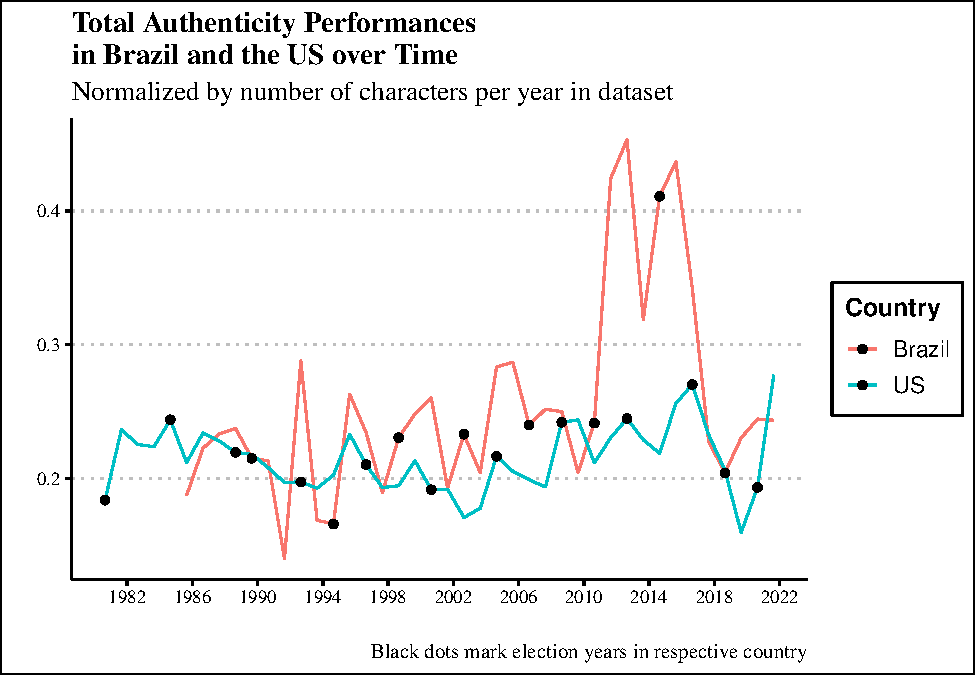
\includegraphics{antipc_files/figure-latex/Figure 1-1.pdf}
\caption{Total Authenticity Performances in Time in Brazil and the US}
\end{figure}

Nevertheless, authenticity has generally been performed with greater
frequency in politics in Brazil since the mid-1990s in comparison to the
US, which could be related to the differences in the number of parties
in the political system. Brazil features many parties and, thus,
politicians are less susceptible to broad party pressure to conform and
represent interests of heterogenous groups within it, in comparison the
US with two major parties. In the case of Brazil, we also see a large
increase in frequencies of authenticities performed between 2011 and
2016, the Dilma Rousseff years \footnote{ A linear regression
  correlating the total of authenticity performances to years, as
  factors, in Brazil confirms statistically significant increases for
  the years of 2012 and 2015, non-election years and when Rousseff was
  president.}. This might indicate a relationship between gender and the
frequencies at which authenticity is performed in politics. However,
there only two women politicians in the sample (Dilma Rousseff and
Hillary Clinton), which makes it challenging to extrapolate how gender
and authenticity performances correlate. Though women in politics have a
distinct communication style than men (Wood 1994; Christine Banwart and
McKinney 2005; Blankenship and Robson 1995; Franceschet, Piscopo, and
Thomas 2016). Rousseff, arguably, needed to justify herself and her
public policies with further concrete reasoning and perform certain
authenticities to connect with audiences more frequently than the men in
the sample. As well, Rousseff is, arguably, the only non-professional
politician elected president of Brazil. Having gone through several high
level techno-bureaucratic positions, Dilma ran for office the first time
in 2010, being elected president.

Notwithstanding, the types of authenticity performed in also politics
change over time. Figure 2, below, illustrates how collective and
individual authenticity performances have changed in time for Brazil and
the US. In the figure, the x-axis represents the years and the y-axis
represents the sum of individual and collective authenticity
performances. In Brazil, collective authenticity performances were
performed considerably more frequently than individual performances from
the 1980s until the early-2010s. This trend began to change at that
point and, by 2019, we see a reversal of this pattern whereas individual
authenticity performances surpass collective performances. Conversely,
in the case of the US, individual authenticity performances were
performed more frequently throughout the 1980s. From the early-1990s
until the early-2010s, both performances appear at very similar rates in
the US. This pattern changed in the mid-2010s with collective
authenticity performances surpassing individual. These changes relate to
background contextual conditions that make some types of performances
more, or less, credible to audiences in each case at certain points in
time. Audiences in Brazil, arguably, became tired of collective
authenticity performances that focused on share cultural links with the
politico-economic crisis of the mid-2010s and, in turn, became more
interested in simpler individual performances that were credible based
on expectations for political performers. In the US, instead, audiences
arguably grew tired of performances that were balanced and focus on both
collective and individual authenticities equally around the early-2010s
in favor performers and/or performances that focused on shared cultural
connections. In both cases, these patterns began to change before most
recent elections (2016 for the US and 2018 for Brazil) and continue
after even as politicians at the top might have changed. This indicates
that timing could favor certain candidates who already perform certain
authenticities, but also that politicians adapt to perform
authenticities that audiences ``want to hear'' at certain times.

\begin{figure}
\centering
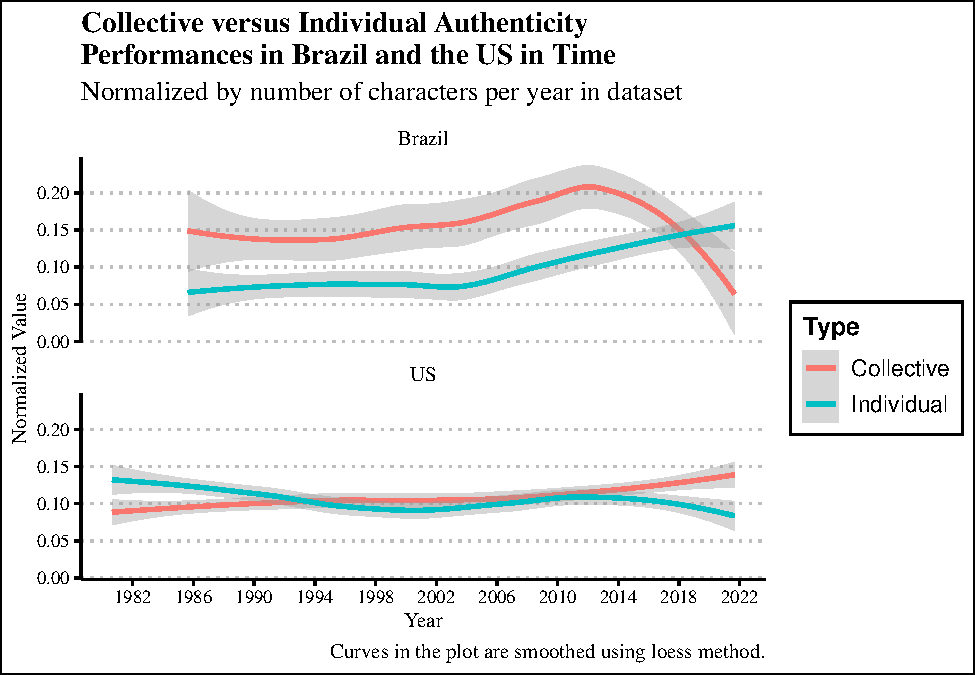
\includegraphics{antipc_files/figure-latex/Figure 2-1.pdf}
\caption{Collective versus Individual Authenticity Performances in Time
in Brazil and the US}
\end{figure}

\hypertarget{authenticity-performances-by-politicians-in-brazil-and-the-us}{%
\subsection{Authenticity Performances by Politicians in Brazil and the
US}\label{authenticity-performances-by-politicians-in-brazil-and-the-us}}

Presidents and presidential candidates focus on some authenticity
performances over others. Figure 3, below, captures authenticity
performances by presidents and presidential candidates that fall above
the 95th percentile in a certain year. In the figure, the x-axis
represents the years and the dots represent a politician that performed
authenticities above the 95th percentile in that year. The 95th
percentiles are calculated for each authenticity performance and for the
total of authenticity performances. Most politicians in Brazil and the
US performed one, or more, authenticities above the 95th percentile when
they were candidates, before being elected the first time (e.g.~Lula),
or after having left office (e.g.~Clinton). This corroborates that
politicians running for re-election perform authenticity less
frequently. Other politicians do not perform any authenticity at the
95th percentile for any year campaigning or in office (e.g.~Reagan and
Cardoso). This indicates that these politicians either perform
authenticity less than others in general and/or that they do not focus
on one authenticity more than other politicians at any point in time
\footnote{ Since authenticity performances as lie acusations and figer
  pointing happen, on average, very infrequently the 95th percentile for
  these are not included on Figure 3 to improve visualization.}.

\begin{figure}
\centering
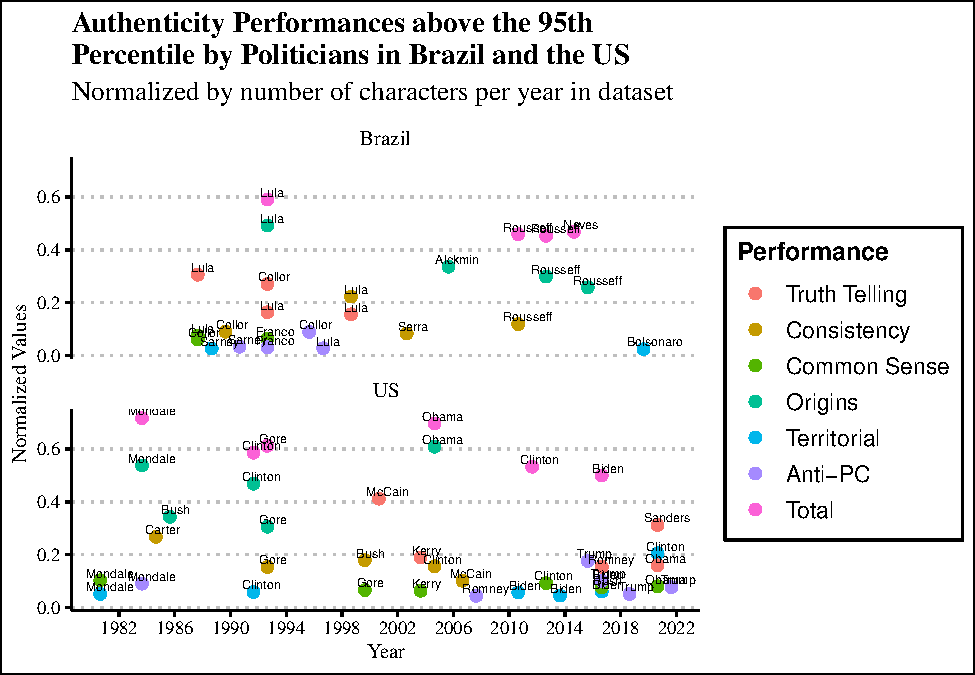
\includegraphics{antipc_files/figure-latex/Figure 3-1.pdf}
\caption{95th Percentile Authenticity Performances by Politicians in
Brazil and the US}
\end{figure}

Moreover, in the case of the US, Mondale, Clinton, Gore, Obama, and H.
Clinton perform the total of authenticity performances above the 95th
percentile at a certain year, but none of these politicians were in the
oval office when they did so. In the case of Brazil, Lula, Collor,
Neves, and Rousseff performed the total of authenticities above the 95th
percentile at a certain year, but only Roussef did so while president.
This is also consistent with Wood (1994) (p.~137-148) argument that
women's speech style in politics include personal disclosures of
details, using of anecdotes, and concrete reasoning, which are
compatible with common sense, consistency, and origins performances that
were performed above the 95th percentile during her years in office. The
fact that Rousseff performed various authenticities in the 95th
percentile while in office further indicates that women in politics have
a distinct style and that they likely feel the need perform authenticity
at a higher rate to connect to audiences and justify policy choices than
their male counterparts.

Associated and opposing politicians often perform the same
authenticities in similar years. Take, for example, the case of anti-PC
in Brazil which was performed by diverse politicians above the 95th
percentile from the early to mid-1990s. Anti-PC in the US, however, was
performed by Mondale in the 1980s and Trump from 2015 onwards
\footnote{Though Trump and Mondale politicians belonged to different
  parties and had divergent political stands, both often employed a
  ``telling like it is'' communication style. For more on Modale's
  ``truth'' telling style see his
  \href{https://www.nytimes.com/1984/07/20/us/transcript-of-mondale-address-accepting-party-nomination.html}{1984}
  Democratic Convention acceptance speech. Some of Mondale's mentions of
  truth telling regarding raising taxes, for example, is similar to
  numerous accounts of Trump's denouncing PC in terms of wasting peoples
  time.}. Indeed, Trump is the only politician the sample who appears to
consistently perform authenticity with anti-PC. Furthermore, in the case
of the US, we also see that truth telling was performed above the 95th
percentile by politicians as Kerry and McCain around the year 2000;
consistency was performed above the 95th percentile in the 2000s by W.
Bush, Clinton, McCain; while origins was performed above the 95th
percentile by Mondale and Bush in the mid-1980s and by Gore and Clinton
in the mid-1990s. Comparably, in the case of Brazil, truth telling,
origins, and consistency were performed above the 95th percentile by
Lula and Collor from the late-1980s to the late-1990s. Similar
authenticity performances above the 95th percentile for associated and
opposing politicians in similar years indicate politicians respond to,
or imitate, each other on specific authenticity performances at a
certain election cycle or connected to background context that make
certain authenticity performance more credible at certain times. This is
especially pertinent as the same politicians often perform different
authenticities above the 95th percentile over time.

\hypertarget{authenticity-performances-across-settings-in-brazil-and-the-us}{%
\subsection{Authenticity Performances across settings in Brazil and the
US}\label{authenticity-performances-across-settings-in-brazil-and-the-us}}

The frequency of authenticity performances changes across settings in
which politics gets done. Figure 4, below, illustrates authenticity
performances in Brazil and the US across setting over time. The x-axis
represents the years and the y-axis represents the sum of all normalized
authenticity performances for each setting per year. The plot shows
that, in the US, authenticity was performed much more frequently in
campaign rallies than in all other settings until mid-2000s \footnote{
  The relationship between the average frequencies of authenticity
  performances per year and setting was also investigated employing
  fixed-effects linear panel models. Fixed-effects models account for
  time effects while controlling for unobserved associations within the
  model variables (Allison 2009). In the regression (see appendix 2),
  the correlation between the frequencies of authenticity performances
  and campaign settings for the US, in comparison to official speeches
  (reference category), is positive and highly statistically
  significant. Interviews also appear to correlate positively with
  authenticity performances in the US, in comparison to official
  speeches. In the case of Brazil, both campaign and debate settings
  correlate positively with authenticity performances in relation to
  official speeches. However, using this approach, we miss how these
  correlations change in time.}. At that point, the frequency in which
authenticity was performed across all settings in the US becomes similar
until the early-2010s, when performances in debates increase while
performances on interviews decrease in frequency. In the case of Brazil,
we see a different trend. The frequency at which authenticity is
performed in campaign rallies generally increased from the late 1980s to
the mid-2010s. In fact, there is a sharp increase in the frequency in
which authenticity is performed in campaign rallies, debates, and
official speeches around the Rousseff years. We also see a sharp
decrease in the frequency in which authenticity is performed across all
setting from the mid-2010s onwards in Brazil.

\begin{figure}
\centering
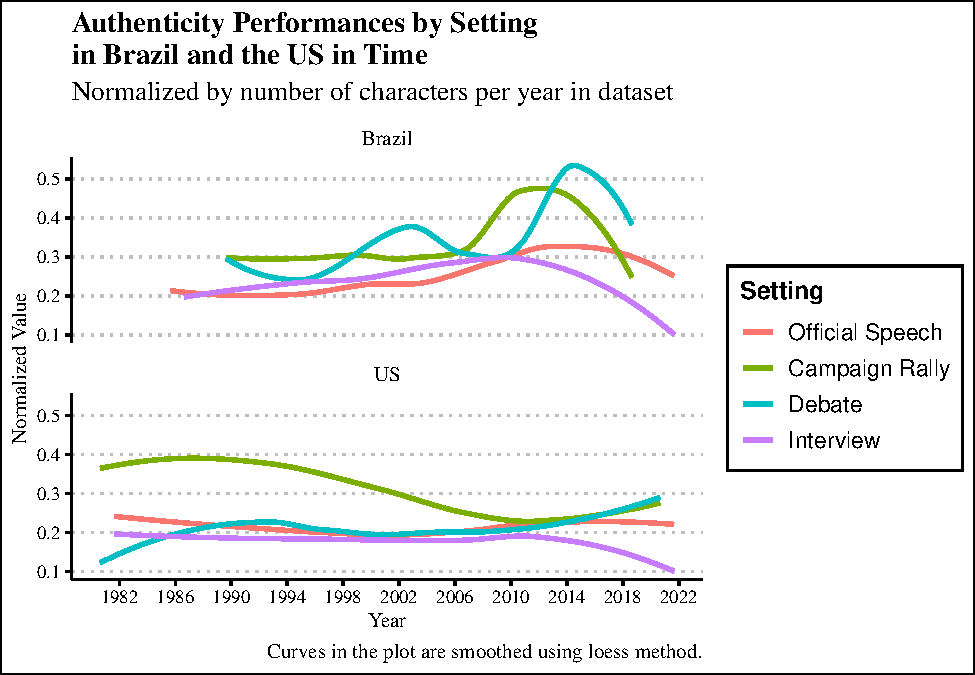
\includegraphics{antipc_files/figure-latex/Figure 4-1.pdf}
\caption{Authenticity Performances by Setting Time in Brazil and the US}
\end{figure}

In both Brazil and the US debates have become the setting in which
authenticity is performed most frequently, whereas interviews are the
setting in which authenticity is performed least frequently, from the
2010 onwards. In the case of interviews, the spread of social media gave
politicians alternative outlets to interact directly with audiences,
bypassing journalists and their filtering (see Alexander 2011, 106),
while performing authenticity directly to wide portions of the
electorate. As for debates, in the case of the US, they went from being
the setting in which authenticity was least performed in the early-1980s
to the setting in which it was most performed by the late-2010s. Debates
also became the setting in which authenticity is most performed in
Brazil by the mid-2010s. In terms of authenticity performances, debates'
format requires candidates to answer quick to sometimes unpredictable
questions and, as large-scale media events, become sources of ``sticky''
sound, text, and video bites charged with imagery, rather than meaning,
that circulate to mark and represent political cycles in democracies
(Foley 2012,; Coleman 2000) \footnote{Though why and the extent to which
  debates might matter for election outcomes is contentious (see
  McKinney and Warner 2013).}. As political bites become shorter, but
more reproduced, debates become ever important settings for a wide
variety of authenticity performances.

\hypertarget{conclusion}{%
\section{Conclusion}\label{conclusion}}

This article set to investigate how anti-PC discourses appear and change
over time in politics. A brief review of the populism and cultural
backlash scholarship illustrated how these literatures focus on
particular manifestations of anti-PC discourses by specific leaders.
Instead, this paper argues that anti-PC discourses in politics are
authenticity performances that reduce the perceived link between what
politicians are thinking and what they are saying to audiences. Several
authenticity performances are also theorized. Individual authenticity
performances, for example, derive plausibility from audiences'
expectations about a political performer (or opponent) considering the
information they have. These performances include claims of truth
telling or consistency and lie accusations or finger pointing.
Collective authenticity performances derive plausibility for performance
based on the cultural connections shared between audiences and
performer. These performances include anti-PC, pointing at origins,
allusions to common sense, or claims of territorial knowledge. A
framework for investigating authenticity performances in politics that
focuses on performative displays (what), projections (who, when, and
where), and mechanisms (how) is developed. A dictionary of terms for
investigating authenticity performances in discourses is built based on
the framework. Texts for campaign rallies, debates, interviews, and
official speeches for presidents and presidential candidates in Brazil
and the US since the 1980s were scraped to construct the datasets. This
allowos for the identification, comparison, and analysis of how
authenticity performances change over time, by politicians, and across
political settings.

The analysis reveals that authenticity performances that promote
oneself, as origins and truth-telling, occur with greater frequency on
average than other performances. As well, the total frequencies of
authenticity performances are not systematically greater in election
years in comparison to non-election years. This indicates that
incumbents might be more careful towards when, where, and how
authenticity is performed around election years. Indeed, most
politicians perform authenticities above the 95th percentile when they
are candidates, before being elected a first time, or after having left
office. However, in the case of Brazil, we see a spike in the frequency
authenticity is performed in politics from 2011 to 2016 while Dilma
Rousseff held office. Women in politics, arguably, perform authenticity
more frequently to justify themselves and their public policy choices
than the men in the sample. Moreover, the variation in types of
authenticity performed over time and across cases indicate that
contextual conditions make some types of performances more, or less,
credible to audiences at certain junctures. Many authenticity
performances appear in high frequencies for opposing and associated
candidates in similar years. In such, politicians adapt to perform
authenticities audiences ``want to hear''. Finally, in both cases in
recent years, debates became the setting in which authenticities are
performed most frequently, whereas interviews are the setting in which
authenticity was performed least frequently. Debates are large-scale
media events that produce ``sticky'' political bites charged with
imagery that circulate more than ever in democracies. Relatedly, in
relation to interviews, social media platforms give politicians diverse
outlets to interact directly with audiences, bypassing journalists.

Alexander (2011, 85) argues, that the ``challenge for social performance
is to make its component parts invisible''. For social scientists, the
challenge has always been to understand when, why, and how political
discourses matter in democracies. Politicians do politics. Looking at
politics as performances emphasizes the performer's role, the script,
the stage, and the audience, rather than only focusing on the content
(or an specific interpretation of discursive content), while placing
agency with both audiences and performers. Authenticity performances, as
a framework, offers a less contentious alternative to understand what
discourses, as anti-PC, are, how they change over time, and why they
might matter for political outcomes. Engaging exclusively with meanings
in political discourses can misplace the logic of why electorates, and
politicians, behave as they do, while contributing to further societal
divides by passing on the blame for ``undesirable'' political outcomes
to a lumped group of ``old, uneducated, or poor'' electorates. Even more
worrisome, a misplaced engagement with political discourses might reveal
biased answers to contemporary political issues. As such, alternative
approaches as authenticity performances might be an appealing extra tool
to engage, respond, and break with lumped generalizations about in
politics.

\newpage

\textbf{References}

\hypertarget{refs}{}
\begin{CSLReferences}{1}{0}
\leavevmode\vadjust pre{\hypertarget{ref-alexander2010}{}}%
Alexander, Jeffrey C. 2010. \emph{The Performance of Politics: Obama's
Victory and the Democratic Struggle for Power}. Oxford University Press.

\leavevmode\vadjust pre{\hypertarget{ref-alexander2011}{}}%
---------. 2011. \emph{Performance and Power}. Polity.

\leavevmode\vadjust pre{\hypertarget{ref-alexander2006}{}}%
Alexander, Jeffrey C, Bernhard Giesen, and Jason L Mast. 2006.
\emph{Social Performance: Symbolic Action, Cultural Pragmatics, and
Ritual}. Cambridge University Press.

\leavevmode\vadjust pre{\hypertarget{ref-allison2009}{}}%
Allison, Paul D. 2009. \emph{Fixed Effects Regression Models}. SAGE
publications.

\leavevmode\vadjust pre{\hypertarget{ref-aslanidis2016}{}}%
Aslanidis, Paris. 2016. {``Is Populism an Ideology? A Refutation and a
New Perspective.''} \emph{Political Studies} 64 (1\_suppl): 88--104.

\leavevmode\vadjust pre{\hypertarget{ref-beard1993}{}}%
Beard, Henry, and Christopher Cerf. 1993. \emph{The Official Politically
Correct Dictionary and Handbook}. Villard Books.

\leavevmode\vadjust pre{\hypertarget{ref-berman2011}{}}%
Berman, Paul. 2011. \emph{Debating PC: The Controversy over Political
Correctness on College Campuses}. Delta.

\leavevmode\vadjust pre{\hypertarget{ref-betz2001}{}}%
Betz, Hans-Georg. 2001. {``Exclusionary Populism in Austria, Italy, and
Switzerland.''} \emph{International Journal} 56 (3): 393--420.

\leavevmode\vadjust pre{\hypertarget{ref-blankenship1995}{}}%
Blankenship, Jane, and Deborah C Robson. 1995. {``A {`Feminine Style'}
in Women's Political Discourse: An Exploratory Essay.''}
\emph{Communication Quarterly} 43 (3): 353--66.

\leavevmode\vadjust pre{\hypertarget{ref-brinton2005}{}}%
Brinton, Laurel J, and Elizabeth Closs Traugott. 2005.
\emph{Lexicalization and Language Change}. Cambridge University Press.

\leavevmode\vadjust pre{\hypertarget{ref-brubaker2017}{}}%
Brubaker, Rogers. 2017. {``Why Populism?''} \emph{Theory and Society} 46
(5): 357--85.

\leavevmode\vadjust pre{\hypertarget{ref-brubaker2020}{}}%
---------. 2020. {``Populism and Nationalism.''} \emph{Nations and
Nationalism} 26 (1): 44--66.

\leavevmode\vadjust pre{\hypertarget{ref-bush1995}{}}%
Bush, Harold K. 1995. {``A Brief History of PC, with Annotated
Bibliography.''} \emph{American Studies International} 33 (1): 42--64.

\leavevmode\vadjust pre{\hypertarget{ref-bybee2015}{}}%
Bybee, Joan. 2015. \emph{Language Change}. Cambridge University Press.

\leavevmode\vadjust pre{\hypertarget{ref-carlo2018}{}}%
Carlo, Josnei, and Joao Kamradt. 2018. {``Bolsonaro e a Cultura Do
Politicamente Incorreto Na Politica Brasileira.''} \emph{Teoria e
Cultura} 13 (2).

\leavevmode\vadjust pre{\hypertarget{ref-cezar2021}{}}%
Cezar, Rodrigo Fagundes. 2020. {``Brazilian Presidential Speeches from
1985 to July 2020.''} Harvard Dataverse.
\url{https://doi.org/10.7910/DVN/M9UU09}.

\leavevmode\vadjust pre{\hypertarget{ref-chait2015}{}}%
Chait, Jonathan. 2015. {``Not a Very PC Thing to Say.''} \emph{New York
Magazine} 27.

\leavevmode\vadjust pre{\hypertarget{ref-christine2005}{}}%
Christine Banwart, Mary, and Mitchell S McKinney. 2005. {``A Gendered
Influence in Campaign Debates? Analysis of Mixed-Gender United States
Senate and Gubernatorial Debates.''} \emph{Communication Studies} 56
(4): 353--73.

\leavevmode\vadjust pre{\hypertarget{ref-coleman2000}{}}%
Coleman, Stephen. 2000. {``Televised Election Debates.''}
\emph{International Perspectives}.

\leavevmode\vadjust pre{\hypertarget{ref-conway2017}{}}%
Conway, Lucian Gideon III, Meredith A Repke, and Shannon C Houck. 2017.
{``Donald Trump as a Cultural Revolt Against Perceived Communication
Restriction: Priming Political Correctness Norms Causes More Trump
Support.''} \emph{Journal of Social and Political Psychology} 5 (1).

\leavevmode\vadjust pre{\hypertarget{ref-conway2009}{}}%
Conway, Lucian Gideon III, Amanda Salcido, Laura Janelle Gornick, Kate
Ashley Bongard, Meghan A Moran, and Chelsea Burfiend. 2009. {``When
Self-Censorship Norms Backfire: The Manufacturing of Positive
Communication and Its Ironic Consequences for the Perceptions of
Groups.''} \emph{Basic and Applied Social Psychology} 31 (4): 335--47.

\leavevmode\vadjust pre{\hypertarget{ref-d1991}{}}%
D'Souza, Dinesh. 1991. \emph{Illiberal Education: The Politics of Race
and Sex on Campus}. Simon; Schuster.

\leavevmode\vadjust pre{\hypertarget{ref-fairclough2003}{}}%
Fairclough, Norman. 2003. {``'Political Correctness': The Politics of
Culture and Language.''} \emph{Discourse \& Society} 14 (1): 17--28.

\leavevmode\vadjust pre{\hypertarget{ref-farias2001}{}}%
Farias, Edilsom Pereira de. 2001. {``Liberdade de Expressao e
Comunicacao.''}

\leavevmode\vadjust pre{\hypertarget{ref-feldstein1997}{}}%
Feldstein, Richard. 1997. \emph{Political Correctness: A Response from
the Cultural Left}. U of Minnesota Press.

\leavevmode\vadjust pre{\hypertarget{ref-fiorin2008}{}}%
Fiorin, Jose Luiz. 2008. {``A Linguagem Politicamente Correta.''}
\emph{Revista Linguasagem} 1 (1).

\leavevmode\vadjust pre{\hypertarget{ref-foley2012}{}}%
Foley, Megan. 2012. {``Sound Bites: Rethinking the Circulation of Speech
from Fragment to Fetish.''} \emph{Rhetoric and Public Affairs} 15 (4):
613--22.

\leavevmode\vadjust pre{\hypertarget{ref-fordahl2018}{}}%
Fordahl, Clayton. 2018. {``Authenticity: The Sociological Dimensions of
a Politically Consequential Concept.''} \emph{The American Sociologist}
49 (2): 299--311.

\leavevmode\vadjust pre{\hypertarget{ref-franceschet2016}{}}%
Franceschet, Susan, Jennifer M Piscopo, and Gwynn Thomas. 2016.
{``Supermadres, Maternal Legacies and Women's Political Participation in
Contemporary Latin America.''} \emph{Journal of Latin American Studies}
48 (1): 1--32.

\leavevmode\vadjust pre{\hypertarget{ref-freitas2013}{}}%
Freitas, Riva Sobrado de, and Matheus Felipe de Castro. 2013.
{``Liberdade de Expressao e Discurso Do Odio: Um Exame Sobre as
Possiveis Limitacoes a Liberdade de Expressao.''} \emph{Sequencia},
327--55.

\leavevmode\vadjust pre{\hypertarget{ref-goffman1956}{}}%
Goffman, Erving. 1956. {``The Presentation of Self in Everyday Life.
University of Edinburgh.''} \emph{Social Sciences Research Centre}.

\leavevmode\vadjust pre{\hypertarget{ref-goncalves2020}{}}%
Goncalves, Felipe, and Gabriela Goncalves. 2020. {``94.''} \emph{G1
Globo}.

\leavevmode\vadjust pre{\hypertarget{ref-gutmann1994}{}}%
Gutmann, Amy. 1994. {``Multiculturalism: Examining the Politics of
Recognition.''}

\leavevmode\vadjust pre{\hypertarget{ref-hall1994}{}}%
Hall, Stuart. 1994. {``Some "Politically Incorrect" Pathways Through
PC'in Sarah Dunant (Ed.) The War of the Words: The Political Correctness
Debate, 164-183.''} \emph{London: Virago}.

\leavevmode\vadjust pre{\hypertarget{ref-hawkins2009}{}}%
Hawkins, Kirk A. 2009. {``Is Chavez Populist? Measuring Populist
Discourse in Comparative Perspective.''} \emph{Comparative Political
Studies} 42 (8): 1040--67.

\leavevmode\vadjust pre{\hypertarget{ref-hawkins2018}{}}%
Hawkins, Kirk A, and Cristobal Rovira Kaltwasser. 2018. {``Measuring
Populist Discourse in the United States and Beyond.''} \emph{Nature
Human Behaviour} 2 (4): 241--42.

\leavevmode\vadjust pre{\hypertarget{ref-hughes2011}{}}%
Hughes, Geoffrey. 2011. \emph{Political Correctness: A History of
Semantics and Culture}. John Wiley; Sons.

\leavevmode\vadjust pre{\hypertarget{ref-laclau2005}{}}%
Laclau, Ernesto. 2005. \emph{On Populist Reason}. Verso.

\leavevmode\vadjust pre{\hypertarget{ref-loury1994}{}}%
Loury, Glenn C. 1994. {``Self-Censorship in Public Discourse: A Theory
of {`Political Correctness'} and Related Phenomena.''} \emph{Rationality
and Society} 6 (4): 428--61.

\leavevmode\vadjust pre{\hypertarget{ref-mckinney2013}{}}%
McKinney, Mitchell S, and Benjamin R Warner. 2013. {``Do Presidential
Debates Matter? Examining a Decade of Campaign Debate Effects.''}
\emph{Argumentation and Advocacy} 49 (4): 238--58.

\leavevmode\vadjust pre{\hypertarget{ref-mishra2017}{}}%
Mishra, Pankaj. 2017. \emph{Age of Anger: A History of the Present}.
Macmillan.

\leavevmode\vadjust pre{\hypertarget{ref-moffitt2016}{}}%
Moffitt, Benjamin. 2016. \emph{The Global Rise of Populism: Performance,
Political Style, and Representation}. Stanford University Press.

\leavevmode\vadjust pre{\hypertarget{ref-moffitt2014}{}}%
Moffitt, Benjamin, and Simon Tormey. 2014. {``Rethinking Populism:
Politics, Mediatisation and Political Style.''} \emph{Political Studies}
62 (2): 381--97.

\leavevmode\vadjust pre{\hypertarget{ref-montanaro2018}{}}%
Montanaro, Domenico. 2018. {``Warning to Democrats: Most Americans
Against US Getting More Politically Correct.''} NPR.

\leavevmode\vadjust pre{\hypertarget{ref-morato2017}{}}%
Morato, Edwiges, and Anna Christina Bentes. 2017. {``{`O Mundo Ta
Chato'}: Algumas Notas Sobre a Dimensao Sociocognitiva Do Politicamente
Correto Na Linguagem.''} \emph{Revista USP}, no. 115: 11--28.

\leavevmode\vadjust pre{\hypertarget{ref-mounk2018}{}}%
Mounk, Yascha. 2018. {``Americans Strongly Dislike PC Culture.''}
\emph{The Atlantic} 10.

\leavevmode\vadjust pre{\hypertarget{ref-mudde2004}{}}%
Mudde, Cas. 2004. {``The Populist Zeitgeist.''} \emph{Government and
Opposition} 39 (4): 541--63.

\leavevmode\vadjust pre{\hypertarget{ref-mudde2007}{}}%
---------. 2007. \emph{Populist Radical Right Parties in Europe}.
Cambridge: Cambridge university press.

\leavevmode\vadjust pre{\hypertarget{ref-norris2019}{}}%
Norris, Pippa, and Ronald Inglehart. 2019. \emph{Cultural Backlash:
Trump, Brexit, and Authoritarian Populism}. Cambridge University Press.

\leavevmode\vadjust pre{\hypertarget{ref-possenti1995}{}}%
Possenti, Sirio. 1995. {``A Linguagem Politicamente Correta e a Analise
Do Discurso.''} \emph{Revista de Estudos Da Linguagem} 3 (2): 123--40.

\leavevmode\vadjust pre{\hypertarget{ref-ragin1987}{}}%
Ragin, Charles C. 1987. \emph{The Comparative Method: Moving Beyond
Qualitative and Quantitative Strategies}. JSTOR.

\leavevmode\vadjust pre{\hypertarget{ref-rosenblum2020}{}}%
Rosenblum, Michael, Juliana Schroeder, and Francesca Gino. 2020. {``Tell
It Like It Is: When Politically Incorrect Language Promotes
Authenticity.''} \emph{Journal of Personality and Social Psychology} 119
(1): 75.

\leavevmode\vadjust pre{\hypertarget{ref-sposito2021}{}}%
Sposito, Henrique. 2021. \emph{Poldis: Tools for Analyzing Political
Discourse}. \url{https://github.com/henriquesposito/poldis}.

\leavevmode\vadjust pre{\hypertarget{ref-stiers2021}{}}%
Stiers, Dieter, Jac Larner, John Kenny, Sofia Breitenstein, Florence
Vallee-Dubois, and Michael Lewis-Beck. 2021. {``Candidate
Authenticity:'to Thine Own Self Be True'.''} \emph{Political Behavior}
43 (3): 1181--1204.

\leavevmode\vadjust pre{\hypertarget{ref-tamaki2020}{}}%
Tamaki, Eduardo Ryo, and Mario Fuks. 2020. {``Populism in Brazil's 2018
General Elections: An Analysis of Bolsonaro's Campaign Speeches.''}
\emph{Lua Nova: Revista de Cultura e Politica}, 103--27.

\leavevmode\vadjust pre{\hypertarget{ref-taylor1992}{}}%
Taylor, Charles. 1992. \emph{The Ethics of Authenticity}. Harvard
University Press.

\leavevmode\vadjust pre{\hypertarget{ref-valgarosson2021}{}}%
Valgarosson, Viktor Orri, Nick Clarke, Will Jennings, and Gerry Stoker.
2021. {``The Good Politician and Political Trust: An Authenticity Gap in
British Politics?''} \emph{Political Studies} 69 (4): 858--80.

\leavevmode\vadjust pre{\hypertarget{ref-dijk1997}{}}%
Van Dijk, Teun A et al. 1997. {``What Is Political Discourse
Analysis.''} \emph{Belgian Journal of Linguistics} 11 (1): 11--52.

\leavevmode\vadjust pre{\hypertarget{ref-weigel2016}{}}%
Weigel, Moira. 2016. {``Political Correctness: How the Right Invented a
Phantom Enemy.''} \emph{The Guardian} 30: 2016.

\leavevmode\vadjust pre{\hypertarget{ref-wc2014}{}}%
Weinmann, Amadeu de Oliveira, and Fabio Vacaro Culau. 2014. {``Notas
Sobre o Politicamente Correto.''} \emph{Estudos e Pesquisas Em
Psicologia} 14 (2): 628--45.

\leavevmode\vadjust pre{\hypertarget{ref-weyland2001}{}}%
Weyland, Kurt. 2001. {``Clarifying a Contested Concept: Populism in the
Study of Latin American Politics.''} \emph{Comparative Politics}, 1--22.

\leavevmode\vadjust pre{\hypertarget{ref-wood1994}{}}%
Wood, Julia T. 1994. {``Gendered Media: The Influence of Media on Views
of Gender.''} \emph{Gendered Lives: Communication, Gender, and Culture}
9: 231--44.

\end{CSLReferences}

\textbf{Appendix}

\begin{landscape}

\begingroup\fontsize{7}{9}\selectfont

\begin{longtabu} to \linewidth {>{\raggedright\arraybackslash}p{2cm}>{\raggedright\arraybackslash}p{6cm}>{\raggedright\arraybackslash}p{8cm}}
\caption{\label{tab:appendix 1}Authenticity Performances Codebook}\\
\toprule
Authenticity Performance & Lexicon English & Lexicon Portuguese\\
\midrule
\endfirsthead
\caption[]{Authenticity Performances Codebook \textit{(continued)}}\\
\toprule
Authenticity Performance & Lexicon English & Lexicon Portuguese\\
\midrule
\endhead

\endfoot
\bottomrule
\endlastfoot
\textbf{Truth Telling} & am telling the truth, are telling the truth, is telling the truth, the truth is, this is the truth, not lying, not lies, no lies, not telling you lies, is honest, am honest, is being honest, are being honest, are honest, honesty, is sincere, are sincere, am sincere, is being sincere, are being sincere, is true, are true, not a liar, bottom of my heart, I swear, I reassure, we reassure, I assure, we assure, be assured, is truthful, are truthful, am truthful, is being truthful, are being truthful, I know that, is evident, are evident, I am sure, trust me, am frank, are frank, is frank, being frank, is upfront, are upfront, am upfront, being upfront, will come clean, am coming clean, are coming clean, is straightforward, are straightforward, being straightforward, believe me, I am certain, no bullshit, not bullshitting & a verdade e, esta e a verdade, digo a verdade, dizemos a verdade, pura verdade, n<U+00E3>o e mentira, n<U+00E3>o estou mentindo, e honesto, sou honesto, somos honesto, sendo honesto, a honestidade, ser sincero, e sincero, com sinceridade, e verdade, s<U+00E3>o verdadeiras, n<U+00E3>o sou mentiroso, n<U+00E3>o minto, fundo do meu cora<U+00E7><U+00E3>o, sou verdadeiro, somos verdadeiros, tenho certeza, certeza absoluta, confia em mim, confie em mim, pode confiar, sou franco, somos francos, fraqueza, falando a verdade, falo a verdade, falamos a verdade, acredite em mim, pode acreditar, podem acreditar, eu tenho certeza, isso e a verdade, somos honestos, com honestidade, toda a sinceridade, com sinceridade, toda sinceridade, sou confi<U+00E1>vel, somos confi<U+00E1>veis, as coisas s<U+00E3>o assim, a realidade das coisas, juro por deus, com certeza, digo com precis<U+00E3>o, veracidade, premissa, afirmo para voc<U+00EA>s, isso e como aconteceu, falar umas verdades\\
\textbf{lying accusations} & not truth, not the truth, not true, aren<U+2019>t true, isn<U+2019>t true, being untruthful, is lying, are lying, is a liar, are liars, is dishonest, are  dishonest, being dishonest, is fake, are fake, being fake, is corrupt, are corrupt, full of lies, not sincere, not being sincere, isn<U+2019>t sincere, aren<U+2019>t sincere, not honest, not being honest, is cheating, is a cheater, are cheaters, are cheating, are tricking, is tricking, be deceived, is deceiving, are deceiving, are a hypocrite, is a hypocrite, are being a hypocrite, is being a hypocrite, is crooked, are crooked, is misleading, are misleading, has double-standards, are sneaky, is sneaky,  has two faces, two-faced, has double faces, double-faced, you are wrong, not correct, fooled by, do not believe, is misrepresenting, they misrepresent, is misrepresent, are misrepresent, pretends that, pretends to, is pretending, are pretending, keep pretending, breach your trust, breach of trust, is false, are false, being false, is misinforming, are misinforming, being misinformed, pretended, cut the crap, full of crap & n<U+00E3>o e verdade, n<U+00E3>o e verdadeiro, e mentiroso, est<U+00E1> mentindo, s<U+00E3>o mentiroso, e mentira, de mentira, tudo mentira, e desonesto, mentiram, mentiu, um desonesto, esse desonesto, de desonesto, s<U+00E3>o desonesto, e falso, s<U+00E3>o falsos, s<U+00E3>o corruptos, e corrupto, de corrupto, todos corrupto, n<U+00E3>o s<U+00E3>o sincero, n<U+00E3>o e sincero, n<U+00E3>o s<U+00E3>o honestos, n<U+00E3>o e honesto, s<U+00E3>o trapaceiros, e trapaceiro, eles trapaceiam, trapaceou, e enganar, ser enganado, v<U+00E3>o enganar, sendo enganados, e hip<U+00F3>crita, e enganador, e engana<U+00E7><U+00E3>o, duas caras, enganado por, n<U+00E3>o acredite, eles finge, ele finge, e fingimento, ela finge, quebrou a sua confian<U+00E7>a , quebra de confian<U+00E7>a,  e falso, s<U+00E3>o falsos, falsidade, e fic<U+00E7><U+00E3>o, hist<U+00F3>ria para boi dormir, historinha para boi dormir, e calunia, s<U+00E3>o calunias, difama<U+00E7><U+00E3>o, difamar, uma inverdade, s<U+00E3>o inverdades, e inverdade, isso e inven<U+00E7><U+00E3>o, essas s<U+00E3>o inven<U+00E7><U+00F5>es, isso e uma lenda, essas s<U+00E3>o ledas, tenta iludir, tentando iludir, uma farsa, tramoia, mal intencionado, mas inten<U+00E7><U+00F5>es, falta de informa<U+00E7><U+00E3>o, esta mal-informado, est<U+00E3>o mal-informados\\
\textbf{Consistency} & we delivered, I delivered, check and see, I keep my word, we keep our word, I kept my word, we kept our word, I keep my promise, I kept my promise, we keep our promise, as promised, we kept our promise, am responsible, I take responsibility, we take responsibility, we assume responsibility, we are accountable, we are responsible, our duty, my duty, give my word, giving my word, own up my, owning up my, accept responsibility, accept the blame, recognize my mistakes, admit I was wrong, I made mistakes, I guarantee, we guarantee, I can guarantee, we can guarantee, I promise, we promise, we can prove, I can prove, we proved, I proved, am reliable, rely on me, rely on us, be reassured, you can hold me accountable, you can hold us accountable, see with your own eyes, vote of confidence, our mission, my mission, my commitment, our commitment, during our government, during my government, while I was in charge & n<U+00F3>s entregamos, eu entreguei, veja com seus pr<U+00F3>prios olhos, cumpro minhas palavras, cumprimos nossas palavra, cumpri minha palavra, cumpro minhas promessas, nossas promessa, um compromisso, meu compromisso, tenho um compromisso com, eu sou respons<U+00E1>vel, eu assumo a responsabilidade, n<U+00F3>s somos respons<U+00E1>veis, n<U+00F3>s assumimos a responsabilidade, nosso dever, meu dever, dou minha palavra, fa<U+00E7>o uma promessa, fazer uma promessa, aceitar a responsabilidade, aceito a responsabilidade, aceitamos a responsabilidade, aceitar a culpa, meus erros, que errei, eu errei, eu garanto, eu posso garantir, eu prometo, podemos provar, posso provar, provaremos, eu provei, voto de confian<U+00E7>a, encarrego pessoalmente, encarreguei pessoalmente, estou comprometido, meu comprometimento, comprometimento com, o comprometimento, fazer o poss<U+00ED>vel, minha supervis<U+00E3>o, minha miss<U+00E3>o, nossa miss<U+00E3>o, no meu governo, no nosso governo, durante nosso governo, eu era encarregado, eu era o encarregado, fomos encarregados de\\
\textbf{Finger Pointing} & are inconsistent, is inconsistent, being inconsistent, are irresponsible, is irresponsible, being irresponsible, their fault, not my fault, not our fault, they left us with, they are responsible, are not responsible, aren<U+2019>t responsible, is not responsible, isn<U+2019>t responsible, costed us, false promises, lack accountability, lacking accountability, not kept their word, not kept his word, not kept her word, not kept promises, not kept the, not kept his, not kept her, not kept their, not keep their word, not keep his word, not keep her word, not keep the, didn<U+2019>t keep the, didn<U+2019>t keep her, didn<U+2019>t keep his, hasn<U+2019>t kept his, hasn<U+2019>t kept her, not recognize, he made mistakes, she made mistakes, they made mistakes, not our mistake, not my mistake, not take responsibility, not my responsibility, not accountable, him accountable, them accountable, her accountable, blame them, blame him, blame his, blame her, their blame, break promises, broken promises, has betrayed, they betrayed, betraying, will betray, has tricked, has lied, not deliver, didn<U+2019>t deliver, hasn<U+2019>t deliver, failed your obligations, failed in your obligations, failed his obligations, failed her obligations, failed in his duty, failed in her duty, failed his duty, failed her duty, failed your duties, stabbed in the back & e inconsistente, s<U+00E3>o inconsistente, e irrespons<U+00E1>vel, s<U+00E3>o irrespons<U+00E1>veis, culpa deles, a culpa n<U+00E3>o e minha, n<U+00E3>o e minha culpa, eles n<U+00F3>s deixaram, s<U+00E3>o respons<U+00E1>veis, e respons<U+00E1>vel, n<U+00F3>s custou, falsas promessas, falta de presta<U+00E7><U+00E3>o de contas, falharam, falhou, n<U+00E3>o cumpriu, n<U+00E3>o cumpriram, n<U+00E3>o reconheceu, n<U+00E3>o reconheceram, errou, erraram, n<U+00E3>o se responsabiliza, n<U+00E3>o me responsabilizo, culpa e sua, sua culpa, quebrar promessas, promessas quebradas, quebra de promessas, fala uma coisa e faz outra, fala uma coisa aqui e faz outra, falsas promessas, s<U+00E3>o trapaceiros, cometeu erros, cometeram erros, n<U+00E3>o reconhece, n<U+00E3>o reconheceu, assumiu a responsabilidade, promete uma coisa, promete o mundo, traiu a confian<U+00E7>a, traiu a sua confian<U+00E7>a, quebra de confian<U+00E7>a, quebraram sua confian<U+00E7>a, e falcatrua, foi falcatrua, cheio de falcatrua, houve fraude, houveram fraudes, fraudulento, uma negociata, facada nas costas, faltou com respeito, n<U+00E3>o faz o que promete, n<U+00E3>o fez o que promete, promessas em v<U+00E3>o, palavras em v<U+00E3>o, falta de comprometimento, falta de compromisso, houveram desvio, houve desvio, a culpa e do, cheio de promessas, a conta n<U+00E3>o fecha, n<U+00E3>o terminaram\\
\textbf{Origins} & I was born, I come from, we come from, I grew up, growing up in, my parents, my mom, my mother, my father, my dad, my family, raised me, I was raised, we were raised, we grew up, my background, being surrounded by, being exposed to, my siblings, going to school in, our local church, Sunday mass, Saturday mass, family tradition, tradition in my house, in our house, growing up, back in the day, my grandparents, in my town, in my state, in my region, our community, in my community, our town, our state, my hometown, our hometown, my home state, our home state, back home, our house, my house, our neighbourhood, in my district, I lived in, we lived in, we used to play, I used to play, I was thought & Eu nasci, Eu vim de, eu venho de, viemos de, cresci, n<U+00F3>s crescemos, meus pais, minha m<U+00E3>e, minha m<U+00E3>e, minha fam<U+00ED>lia, fui criado, fomos criados, minhas origens, meus irm<U+00E3>os, meu irm<U+00E3>o, minha irm<U+00E3>, tradi<U+00E7><U+00E3>o familiar, tradi<U+00E7><U+00E3>o em casa, crescendo, antigamente, meu av<U+00F4>, minha av<U+00F3>, meus av<U+00F3>s, na minha cidade, no meu estado, na minha regi<U+00E3>o, nossa comunidade, na minha comunidade, nossa cidade, nosso estado, cidade natal, estado de origem, minha casa, nossa casa, l<U+00E1> em casa, nosso bairro, no meu bairro, eu morava, viv<U+00ED>amos, na minha terra, de onde eu venho, missa de domingo, missa toda semana, brincava, eram outros tempos, fui educado, mor<U+00E1>vamos, eu morei, n<U+00F3>s moramos, de onde venho, eram tempos diferentes\\
\addlinespace
\textbf{Common Sense} & is common sense, are common sense, everyone knows, it is undeniable, stating the obvious, say the obvious, everyone agrees, we all know, common wisdom, the people know, popular knowledge, from experience, it is my experience, sound judgment, practical solution, practical choice, practical answer, pragmatic solution, pragmatic answer, pragmatic choice, realistic answer, let me tell you about, is obvious, are obvious, obvious answer, obvious solution, as we all learned, we have all learned that, do not need to tell you that, the reality is, there is no logic, it does not make sense, it doesn<U+2019>t make sense, we know it does not work, no one disagrees that, no person disagrees, there is not a person, there is not a human being, there is not a family, there is not an American, there is no single citizen, there is not one single person, there is not one single human being, there is not one single family, there is not one single American, there is not one single citizen, there is not one single person, there is not one human being, there is not one family, there is not one American & senso comum, bom senso, todos sabem, afirmando o <U+00F3>bvio, todos concordam, todos sabemos, sabemos todos, todos n<U+00F3>s sabemos, sabedoria popular, por experi<U+00EA>ncia, e minha experi<U+00EA>ncia, sou pr<U+00E1>tico, tem que ser pr<U+00E1>tico, devemos ser pr<U+00E1>tico, sendo pr<U+00E1>tico, sou pragm<U+00E1>tico, tem que ser pragm<U+00E1>tico, devemos ser  pragm<U+00E1>tico, sendo pragm<U+00E1>tico, sou realista, sendo realista, sejamos realista, realisticamente falando, e <U+00F3>bvio, como todos n<U+00F3>s aprendemos, como sabemos, n<U+00E3>o preciso te dizer, o povo sabe, agente aprendeu, n<U+00F3>s aprendemos, n<U+00F3>s sabemos, n<U+00E3>o tem logica, como aprendemos, n<U+00E3>o faz sentido, n<U+00E3>o fazem sentido, estamos cansados de saber, sabemos que n<U+00E3>o funciona, ningu<U+00E9>m discorda que, n<U+00E3>o tem uma pessoa, n<U+00E3>o existe uma pessoa, n<U+00E3>o h<U+00E1> uma pessoa, n<U+00E3>o existe um ser humano, n<U+00E3>o tem um ser humano, n<U+00E3>o h<U+00E1> um ser humano, n<U+00E3>o tem uma fam<U+00ED>lia, n<U+00E3>o existe uma fam<U+00ED>lia, n<U+00E3>o h<U+00E1> uma fam<U+00ED>lia, n<U+00E3>o tem um brasileiro, n<U+00E3>o h<U+00E1> um Brasileiro, n<U+00E3>o existe um brasileiro, n<U+00E3>o tem uma brasileira, n<U+00E3>o h<U+00E1> uma Brasileira, n<U+00E3>o existe uma brasileira\\
\textbf{Anti-PC} & politically correct, political correctness, PC, plain speaking, speaking my mind, speak my mind, say what I think, saying what I think, not going to pretend, not pretend, speak what you think, not what you want to hear, not butter up, not beat around the bush, cut to the chase, just being real, saying what everyone thinks, say what everyone is thinking, speaking plainly, coloured people, negro, retarded, nigger, third world, oriental people, crippled people, is crippled, culturally deprived, drug addict, junkie, drunk, fat people, fat person, fat population, handicapped, homosexual faggot, deviant, perverted, illegals, illegal immigrants, illegal alien, Jew, non-white, prostitutes, promiscuous, stupid, tribe, underdeveloped & politicamente correto, falar francamente, falando francamente, falar o que penso, falo o que penso, falando o que penso, dizer o que penso, papas na l<U+00ED>ngua, n<U+00E3>o vou fingir, n<U+00E3>o estou aqui para agradar, falar o que voc<U+00EA> pensa, o que voc<U+00EA> quer ouvir, n<U+00E3>o adulterar, n<U+00E3>o rodeio, n<U+00E3>o dou rodeio, direto ao ponto, dizer o que todos pensam, dizendo o que penso, dizendo o que todos pensam, dizer o que todos est<U+00E3>o pensando, n<U+00E3>o vou amaciar, n<U+00E3>o d<U+00E1> para amaciar, gordos, retardado, retardada, veado, popula<U+00E7><U+00E3>o preta, os pretos, as pretas, terceiro mundo, viciado em drogas, b<U+00EA>bado, drogado, sem cultura, pervertidos, prom<U+00ED>scuo, imbecil, estupido, aleijado, defeituoso, incapacitado, inv<U+00E1>lido, mongoloide, deficiente mental, defici<U+00EA>ncia mental, o incapacitado, a incapacitada, travesti, homossexualismo\\
\textbf{Territory} & have been to, have visited, came all the way to, back from, will visit, saw first-hand, see first-hand, we visited, I visited, we visited, travelled to, traveling to, spend a few days in, spent some time in, spent time in, met great people in, we were hosted, I was hosted, our time in, my time in, our visit, spent a lot of time in, were many times in, got to know the whole country, got to know all the states & estive em, visitei, voltou de, voltei de, voltando de, voltamos de, estive em, estivemos em, visitar<U+00E1>, visitarei, vi em primeira m<U+00E3>o, ver em primeira m<U+00E3>o, visitamos, viajei para, passei alguns dias em, passei algum tempo em, passei um tempo, conheci <U+00F3>timas pessoas, conhecemos <U+00F3>timas pessoas em, fomos hospedados, minha passagem, nossa passagem, nossa visita, fui muitas vezes para, estive muitas vezes em, passei muito tempo em, meu tempo em, estive por todo o Brasil, de norte a sul do pais, conhe<U+00E7>o todo o pais, conheci todo o pais, conheci todo o Brasil, conhe<U+00E7>o todo o Brasil\\*
\end{longtabu}
\endgroup{}

\end{landscape}

\begin{table}

\caption{\label{tab:appendix 2}Authenticity Performances by Setting in Brazil and the US}
\centering
\begin{tabular}[t]{lcc}
\toprule
  & Brazil & US\\
\midrule
SettingCampaign Rally & \num{0.086}* & \num{0.087}***\\
 & (\num{0.042}) & (\num{0.020})\\
SettingDebate & \num{0.129}** & \num{-0.005}\\
 & (\num{0.045}) & (\num{0.030})\\
SettingInterview & \num{-0.025} & \num{-0.037}*\\
 & (\num{0.024}) & (\num{0.017})\\
\midrule
Num.Obs. & \num{82} & \num{119}\\
R2 & \num{0.250} & \num{0.337}\\
R2 Adj. & \num{-0.447} & \num{-0.057}\\
AIC & \num{-202.5} & \num{-319.2}\\
BIC & \num{-192.9} & \num{-308.1}\\
RMSE & \num{0.07} & \num{0.06}\\
\bottomrule
\multicolumn{3}{l}{\rule{0pt}{1em}+ p $<$ 0.1, * p $<$ 0.05, ** p $<$ 0.01, *** p $<$ 0.001}\\
\end{tabular}
\end{table}


\bibliographystyle{spphys}
\bibliography{bibliography.bib}


\end{document}
